\documentclass[13pt]{extarticle}

\usepackage[T1]{fontenc}
\usepackage[utf8]{inputenc}
\usepackage[russian]{babel}

% page margin
\usepackage[top=2cm, bottom=2cm, left=2cm, right=2cm]{geometry}

% AMS packages
\usepackage{amsmath}
\usepackage{amssymb}
\usepackage{amsfonts}
\usepackage{amsthm}

\usepackage{float}
\usepackage{graphicx}
\usepackage{tabularx}

\newcommand{\lb}{\left(}
\newcommand{\rb}{\right)}

\makeatletter
\setlength{\@fptop}{0pt}
\makeatother

\begin{document} 

Соль -- $NaBr$. \par
\textit{Предельный закон} Дебая-Хюккеля (первое приближение): 
\begin{gather}
	\lg f_{\pm}^{(N)} = - | z_+ z_- | h \sqrt{J} \notag
\end{gather}

Уравнение Дебая-Хюккеля во втором приближении:
\begin{gather}
	\lg f_{\pm}^{(N)} = - \frac{ | z_+ z_- | h \sqrt{J} }{ 1 + a B \sqrt{J} } \notag
\end{gather}

Постоянные $h$ и $B$ определяются следующими соотношениями:
\begin{gather}
h = \frac{e^3}{8 \pi \varepsilon \varepsilon_0 k T \cdot 2.3036} \sqrt{ \frac{2 \cdot 10^3 N_A }{ \varepsilon \varepsilon_0 k T} } \notag \\
B = e \frac{ 2 \cdot 10^3 N_A }{ \varepsilon \varepsilon_0 k T } \notag
\end{gather}

Найдем параметр $a$ исходя из следующей формы уравнения Дебая-Хюккеля во втором приближении:
\begin{gather}
	1 + a B \sqrt{J} = - \frac{ |z_+ z_-| h \sqrt{J} }{ \lg f_{\pm}^{(N)} } \notag
\end{gather}
В координатах $\displaystyle \sqrt{J} - \frac{ |z_+ z_-| h \sqrt{J} }{ \lg f_{\pm}^{(N)} }$ получим прямую, по угловому коэффициенту которой определим значение параметра $a$.

\begin{figure}[!ht]
\centering
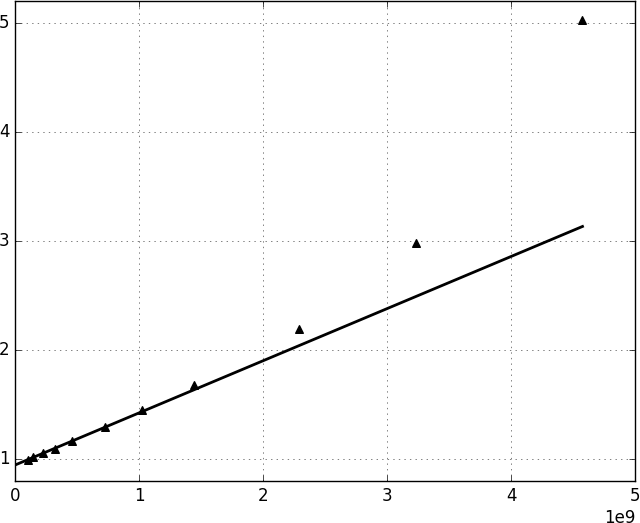
\includegraphics[scale = 0.6]{../pictures/regr.png}
\caption{Нахождение параметра $a$}
\end{figure}

\begin{table}[!ht]
\centering
\begin{tabular}{|c|c|c|c|c|}
\hline
T, K & $\varepsilon$ & $h$, (л/моль)$^{1/2}$ & $B$, (л/моль)$^{1/2}$ / м & $a$, \AA \\
\hline
$298.15$ & $78.3$ & $0.4860$ & $3.236 \cdot 10^9$ & $4.944$ \\
\hline
\end{tabular}
\caption{Параметры уравнения Дебая-Хюккеля}
\end{table}

\begin{figure}[!ht]
\centering
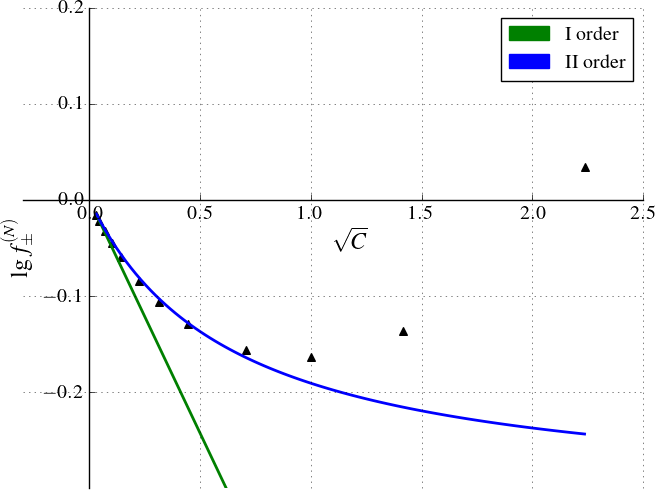
\includegraphics[scale = 0.6]{../pictures/pic1.png}
\caption{Зависимость среднего коэффициента активности от концентрации в водном растворе $NaBr$; 
точками отмечены справочные данные [1]}
\end{figure}

\clearpage

Уравнение Дебая-Хюккеля-Онзагера для эквивалентной электропроводности $\Lambda$ в растворе 1,1-валентного электролита:
\begin{gather}
	\Lambda = \Lambda^0 - (2 b_{ \textup{э} } + b_p \Lambda^0 ) \sqrt{c}, \notag
\end{gather}
где 
\begin{gather}
	b_{\textup{э}} = 4.124 \cdot 10^{-4} \frac{1}{\eta ( \varepsilon T )^{1/2}} \left[ \frac{\textup{См} \cdot \textup{м}^2}{ \textup{г} \cdot \textup{экв} } \cdot \frac{\textup{Н} \cdot \textup{с}}{\textup{м}^2} \cdot \frac{K^{1/2}}{(\textup{г} \cdot \textup{экв}/\textup{л})^{1/2}} \right] \notag \\
	b_p = 8.204 \cdot 10^5 \frac{1}{(\varepsilon T)^{3/2}} \left[ \lb \frac{\textup{г} \cdot \textup{экв} }{\textup{л} } \rb^{-1/2} \textup{К}^{3/2} \right] \notag
\end{gather}

В водных растворах при $T = 298.15$K уравнение Дебая-Хюккеля-Онзагера для 1,1-валентного электролита сводится к:
\begin{gather}
	\Lambda = \Lambda^0 - ( 60.4 \cdot 10^{-4} + 0.23 \Lambda^0 ) \sqrt{c} \notag
\end{gather}


\end{document}